\section{Specific Topologies }

Let $\mathbf{X} \in \mathbb{R}^{D \times N}$ be a sequence of $N$ $D$-dimensional vectors, let $\Lambda$ be a set of symbols and let $\mathbf{H} = g(\mathbf{X})$,  $\mathbf{H} \in \mathbb{R}^{L \times M}$, be the output a weighting function $g$ (e.g. a neural network) which takes $\mathbf{X}$ as input sequence and outputs a sequence of $M$ $|\Lambda|$-dimensional vectors such that $\mathbf{h}_{m} = g_m ( \mathbf{X})$. The weights $\mathbf{H}$ may be interpreted as the weights of a SWFSA whose structure may be defined in various ways. In the rest of this section we explore some commonly used structure for speech recognition. 

\subsection{Time-synchronous WFSA}

Let $\mathbf{H}$ have length  $M = N + 1$ that is for every time step $\mathbf{x}_n$ there is a corresponding weighting vector $\mathbf{h}_n$ and a final weighting $\mathbf{h}_{N+1}$. We define a time-synchronous WFSA over a semiring $K$ as $\mathcal{A} = (\Lambda, \{0, \dots, N \times |\Lambda| \}, \boldsymbol{\alpha}, \mathbf{T}, \boldsymbol{\omega}, \bar{0}, \boldsymbol{\lambda})$ where:

\begin{align}
    \boldsymbol{\alpha} &= \begin{bmatrix} \mathbf{h}_1 \\ \mathbf{0} \end{bmatrix} & \boldsymbol{\omega} &= \begin{bmatrix} \mathbf{0} \\ \mathbf{h}_{N+1} \end{bmatrix} \\
    \mathbf{T} &= \begin{bmatrix}
        \mathbf{0} & \mathbf{1} \mathbf{h}_2^\top & \mathbf{0} & \dots\\
        \mathbf{0} & \mathbf{0} & \mathbf{1} \mathbf{h}_3^\top & \ddots \\
        \vdots & & \ddots & \ddots 
    \end{bmatrix} & \boldsymbol{\lambda} &= \mathbf{1}_{N} \otimes \begin{bmatrix} 
        l_1 \\ \vdots \\ l_{|\Lambda|}
    \end{bmatrix}, \; \forall l \in \Lambda.
\end{align}

\subsubsection{Intersection}
The intersection of a time synchronous WFSA $A$ with an arbitrary WFSA $B$ yields another time-synchronous WFSA $C = A \cap B = (\Lambda, Q_C, \boldsymbol{\alpha}_C, \mathbf{T}_C
, \boldsymbol{\omega}_C, \bar{0}, \boldsymbol{\lambda}_C)$ defined as such:
\begin{align}
    Q &= \{0, 1, \dots, N|\Lambda| \} \\
    \boldsymbol{\alpha}_C &= \begin{bmatrix}
        (\mathbf{M}^\top \mathbf{h}_1) \circ \boldsymbol{\alpha}_B \\ \mathbf{0}
    \end{bmatrix} \qquad \boldsymbol{\omega}_C = \begin{bmatrix}
        \mathbf{0} \\(\mathbf{M}^\top \mathbf{h}_{N+1}) \circ \boldsymbol{\omega}_B 
    \end{bmatrix} \\
    \mathbf{T} &= \begin{bmatrix}
        \mathbf{0} & \mathbf{1} (\mathbf{M}^\top \mathbf{h}_2)^\top \circ \mathbf{T}_B & \mathbf{0} & \dots\\
        \mathbf{0} & \mathbf{0} & \mathbf{1} (\mathbf{M}^\top \mathbf{h}_3)^\top \circ \mathbf{T}_B & \ddots \\
        \vdots & \vdots & \vdots & \ddots 
    \end{bmatrix} \quad \boldsymbol{\lambda} = \begin{bmatrix} 
        \boldsymbol{\lambda}_B \\ \boldsymbol{\lambda}_B \\ \dots
    \end{bmatrix}.
\end{align}
In practice it is usually not necessary to evaluate the elements of $C$ as one can evaluate $W(C)$ directly as follows:
\begin{align}
    \mathbf{u}_1 &= (\mathbf{M}^\top \mathbf{h}_1) \circ \boldsymbol{\alpha}_B \\
    \mathbf{u}_n &= (\mathbf{M}^\top \mathbf{h}_n) \circ (\mathbf{T}_B^\top \mathbf{u}_{n-1}) \\
    W(C) &= \mathbf{u}_N^\top [(\mathbf{M}^\top \mathbf{h}_{N+1}) \circ \boldsymbol{\omega}_B]
\end{align}

\begin{figure}[t] 
    \centering 
    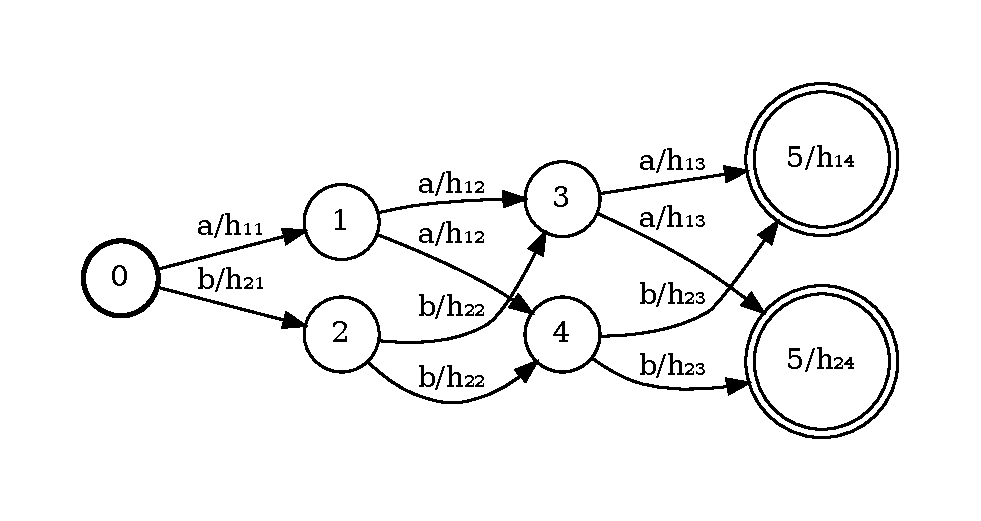
\includegraphics[width=0.7\linewidth]{images/dense.pdf}
    \label{fig:dense_fsa}
\end{figure}

\begin{align}
    \mathbf{v}_{N+1} &= (\mathbf{M}^\top \mathbf{h}_{N+1}) \circ \boldsymbol{\omega}_B \\
    \mathbf{v}_{n} &= \mathbf{T}_B [ (\mathbf{M}^\top \mathbf{h}_n) \circ \mathbf{v}_{n+1}] \\
    W(C) &= [(\mathbf{M}^\top \mathbf{h}_1) \circ \boldsymbol{\alpha}_B]^\top \mathbf{v}_2
\end{align}
Generally, for any $n$, $1 < n < N+1$, 
\begin{align}
    W(C) &= \mathbf{u}_n^\top \mathbf{v}_{n+1}
\end{align}

\paragraph{Gradient}

\begin{align} 
    % \mathbf{g}_{n} &= \mathbf{M}^\top \mathbf{h}_{n} \\
    \mathbf{g}_{n} &= \exp \{ \mathbf{x}_n \} = \mathbf{M}^\top \mathbf{h}_n\\
    \frac{\partial \ln W(C)}{\partial \mathbf{x}_{n}} &= \frac{1}{W(C)} \frac{\partial W(C)}{\partial \mathbf{g}_n} \frac{\partial \mathbf{g}_n}{\partial \mathbf{x}_n} \\ %\frac{\partial \mathbf{h}_n}{\partial \mathbf{x}_n} 
    &= \frac{1}{W(C)} (\mathbf{u}_n \circ \mathbf{v}_{n+1})
\end{align}

\begin{align} 
    \mathbf{h}_n &= \exp \{ \mathbf{x}_n \} \\
    \mathbf{g}_{n} &= \mathbf{M}^\top \mathbf{h}_{n} \\
    \frac{\partial \ln W(C)}{\partial \mathbf{x}_{n}} &= \frac{1}{W(C)} \frac{\partial W(C)}{\partial \mathbf{g}_n} \frac{\partial \mathbf{g}_n}{\partial \mathbf{h}_n} \frac{\partial \mathbf{h}_n}{\partial \mathbf{x}_n} \\
    &= \frac{1}{W(C)} \exp \{ \mathbf{x}_n \} \circ \mathbf{M} \Big( (\mathbf{T}_B^\top \mathbf{u}_{n-1}) \circ \mathbf{v}_{n+1} \Big)
\end{align}

\subsubsection{Current Implementation of $\nabla_\mathbf{H} W(C)$}
\paragraph{Forward Recursion}
\begin{align}
    \mathbf{u}_1 &= \boldsymbol{\alpha}_B \\
    \mathbf{u}_n &= \mathbf{T}_B^\top [ (\mathbf{M}^\top \mathbf{h}_{n-1}) \circ \mathbf{u}_{n-1} ] \\
    W(C) &= [(\mathbf{M}^\top \mathbf{h}_N) \circ \mathbf{u}_N]^\top [(\mathbf{M}^\top \mathbf{h}_{N+1}) \circ \boldsymbol{\omega}_B]
\end{align}

\paragraph{Backward Recursion}
\begin{align}
    \mathbf{v}_{N} &= (\mathbf{M}^\top \mathbf{h}_{N+1}) \circ  \boldsymbol{\omega}_B \\
    \mathbf{v}_n &= \mathbf{T}_B [ (\mathbf{M}^\top \mathbf{h}_{n+1}) \circ \mathbf{v}_{n+1} ] \\
    W(C) &= [(\mathbf{M}^\top \mathbf{h}_1) \circ \boldsymbol{\alpha}_B]^\top \mathbf{v}_1 \\
    W(C) &= [(\mathbf{M}^\top \mathbf{h}_n) \circ \mathbf{u}_n]^\top \mathbf{v}_n
\end{align}

\paragraph{Gradient}
\begin{align}
    \mathbf{h}_n &= \exp\{\mathbf{x}_n\} \\
    \frac{\partial W(C)}{\partial \mathbf{h}_n} &= 
        \frac{\partial}{\partial \mathbf{h}_n}
        [(\mathbf{M}^\top \mathbf{h}_n) \circ \mathbf{u}_n]^\top \mathbf{v}_n \\
    &= \mathbf{M}(\mathbf{u}_n \circ \mathbf{v}_n)\\
    \frac{\partial W(C)}{\partial \mathbf{h}_{N+1}} &= 
        \frac{\partial}{\partial \mathbf{h}_{N+1}}
        [(\mathbf{M}^\top \mathbf{h}_n) \circ \mathbf{u}_n]^\top
        [(\mathbf{M}^\top \mathbf{h}_{N+1}) \circ  \boldsymbol{\omega}_B] \\
    &= \mathbf{M}[(\mathbf{M}^\top\mathbf{h}_N) \circ \mathbf{u}_N \circ \boldsymbol{\omega}_B]\\
    \frac{\partial \log\left(W(C)\right)}{\partial \mathbf{x}_n} &= 
        \frac{\partial \log\left(W(C)\right)}{\partial W(C)}
        \left[
            \frac{\partial \mathbf{h}_n}{\mathbf{x}_n}
        \right]^\top 
        \frac{\partial W(C)}{\partial \mathbf{h}_n}\\
    &= \frac{1}{W(C)} \exp\{\mathbf{x}_n\} \circ \mathbf{M}(\mathbf{u}_n \circ \mathbf{v}_n)
\end{align}